\documentclass{article}
\usepackage[utf8]{inputenc}

\title{\underline{\textit{\Large{ASSIGNMENT 9: SPECTRA OF NON-PERIODIC SIGNAL}}}}
\author{\textit{ROHIT KUMAR, EE20B111}}
\date{\today}

\usepackage{natbib}
\usepackage{graphicx}
\usepackage{amsmath}
\usepackage{listings}

\begin{document}

\maketitle

\section{Abstract}
\begin{itemize}
\item Obtaining the DFT of non-periodic functions.
\item To see how the use of windowing functions (e.g Hamming Window) can help in making the DFT better.
\end{itemize}

\section{Introduction}
In this assignment, we continue our analysis of signals using Fourier Transforms. This time, we focus on finding transforms of non periodic functions. These functions have a discontinuity when periodically extended.\newline 
The discontinuity causes fourier components in frequencies other than the sinusoids frequency which decay as
\(\frac{1}{\omega}\), due to Gibbs phenomenon. We resolve this problem using a hamming window in the case of this assignment.\newline 
We use this windowed transform to analyse signals known to contain a sinusoid of unknown frequencies and extract its phase and frequency. We also perform a sliding DFT on a chirped signal and then plot the results.

\section {Worked Examples}

The worked examples in the assignment are given below:
Spectrum of $sin(\sqrt{2}t)$ is given below\newline
\begin{figure}[h!]
\centering
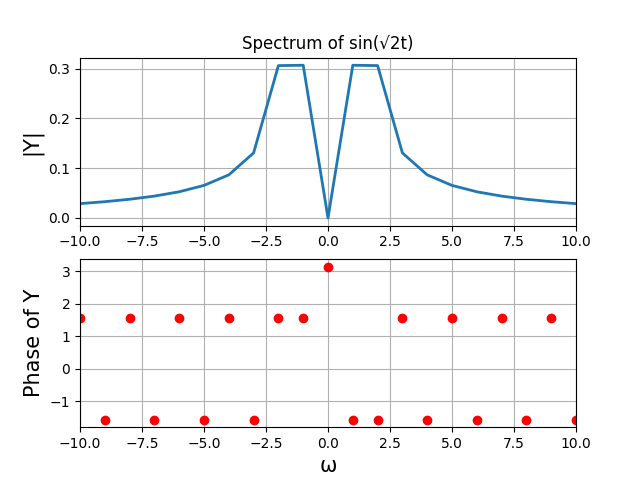
\includegraphics[scale=0.6]{fig10-1.png}
\caption{Spectrum of sin(\sqrt{2}t)}
\label{fig:universe}
\end{figure}
\clearpage
Original function for which we want the DFT:
\begin{figure}[h!]
\centering
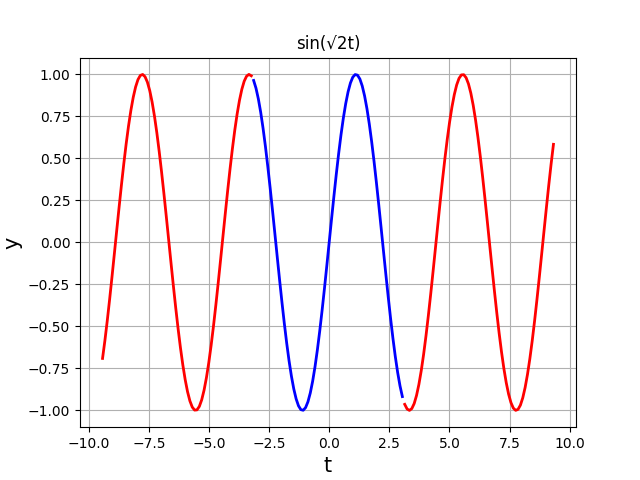
\includegraphics[scale=0.6]{fig10-2.png}
\caption{sin(\sqrt{2}t)}
\label{fig:universe}
\end{figure}

Since the DFT is computed over a finite time interval, We actually plotted the DFT for this function
\begin{figure}[h!]
\centering
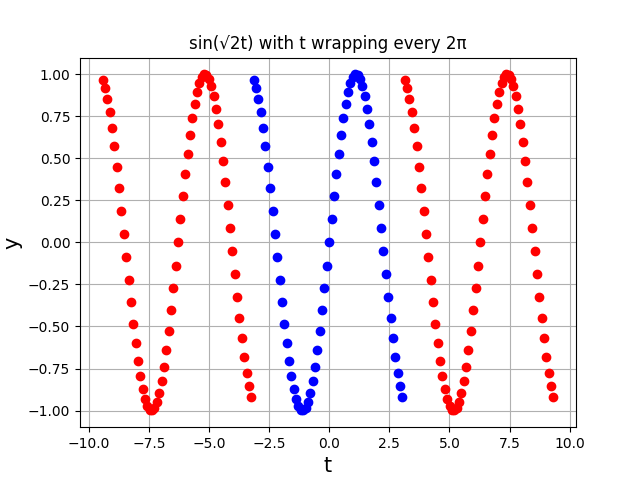
\includegraphics[scale=0.6]{fig10-3.png}
\caption{Spectrum of sin(\sqrt{2}t)}
\label{fig:universe}
\end{figure}

These discontinuities lead to  non harmonic components in the FFT which decay as \(\frac{1}{\omega}\). To confirm
this, we plot the spectrum of the periodic ramp below:
\begin{figure}[h!]
\centering
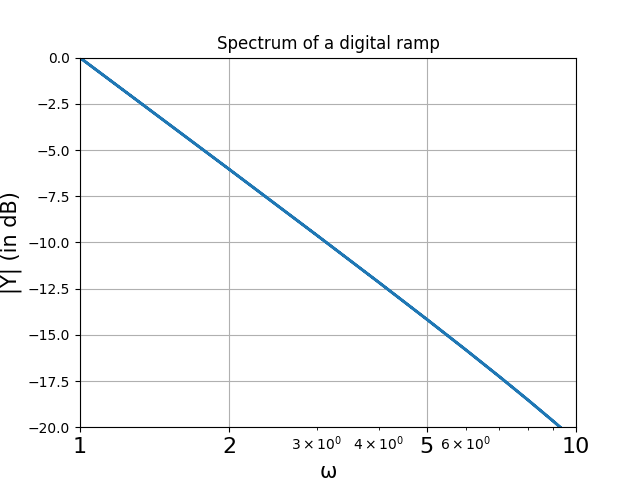
\includegraphics[scale=0.6]{fig10-4.png}
\caption{Spectrum of sin(\sqrt{2}t)}
\label{fig:universe}
\end{figure}

\subsection{Hamming Window}
The hamming window removes discontinuities by attenuating the high frequency components that cause the discontinuities.
The hamming window function is given by
\begin{equation}
    x[n] = 0.54 + 0.46cos(\frac{2\pi n}{N-1})
\end{equation}

We now multiply our signal with the hamming window and periodically extend it. Note that the discontinuities nearly vanish
\begin{figure}[h!]
\centering
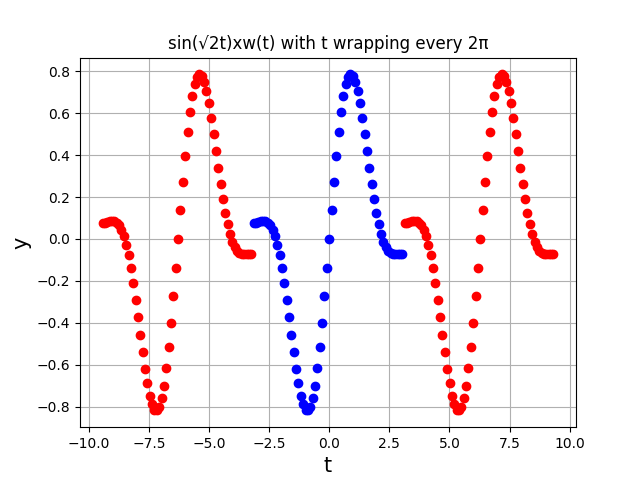
\includegraphics[scale=0.6]{fig10-5.png}
\caption{Spectrum of sin(\sqrt{2}t)*w(t)}
\label{fig:universe}
\end{figure}
\clearpage

The spectrum that is obtained with a time period $2\pi$ is given below:
\begin{figure}[h!]
\centering
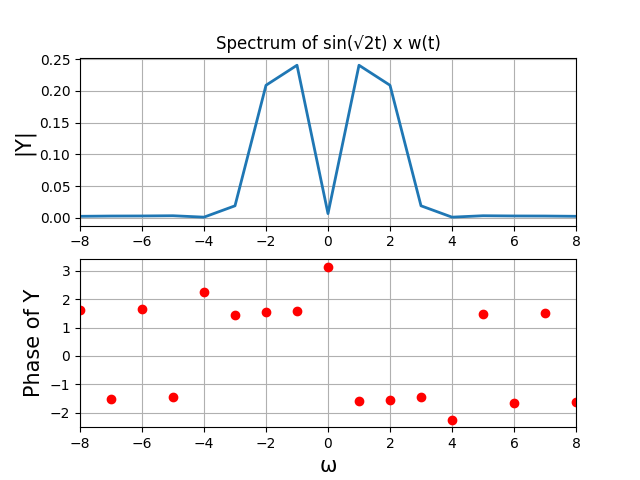
\includegraphics[scale=0.6]{fig10-6.png}
\caption{Spectrum of sin(\sqrt{2}t)*w(t)}
\label{fig:universe}
\end{figure}

The spectrum that is obtained with a time period $8\pi$ has a slightly sharper peak and is given below:
\begin{figure}[h!]
\centering
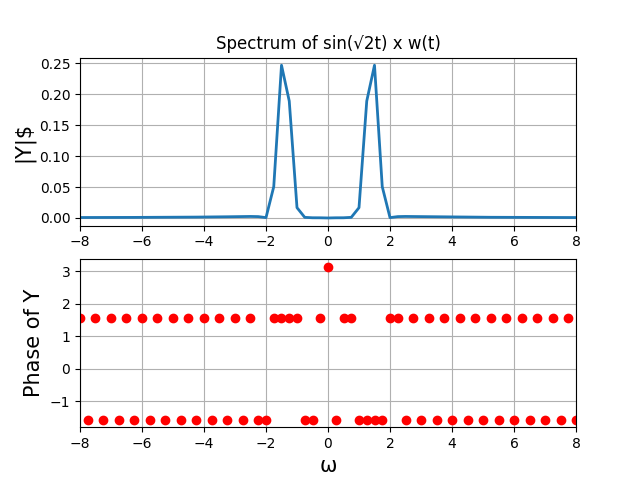
\includegraphics[scale=0.6]{fig10-7.png}
\caption{Spectrum of sin(\sqrt{2}t)*w(t)}
\label{fig:universe}
\end{figure}

\section{Assignment questions}

\subsection{Helper Functions}
Given below is a helper function that plots and returns the DFT of an arbitrary function.

\lstset{language=Python}
\lstset{frame=lines}
\lstset{label={lst:code_direct}}
\lstset{basicstyle=\footnotesize}
\begin{lstlisting}
def spectrum(lim, n, f, t_temp = 0, show_temp = True, t_lims = False, windowing = False, 
xlim1 = 10, title1 = "Spectrum of sin(\u221A2t)", xlabel1 = "\u03C9", ylabel1 = "|Y|", 
ylabel2 = "Phase of Y", savename = "abc.png"):
    if(t_lims):
        t = t_temp
    else:
        t = linspace(-lim, lim, n + 1)[:-1]
    dt = t[1] - t[0]
    fmax = 1/dt
    y = f(t)
    if(windowing):
        m = arange(n)
        wnd = fftshift(0.54 + 0.46*cos(2*pi*m/n))
        y = y*wnd
    y[0] = 0 # The sample corresponding to -tmax should be set to zero
    y = fftshift(y) # Make y start with y(t=0)
    Y = fftshift(fft(y))/float(n)
    w = linspace(-pi*fmax, pi*fmax, n + 1)[:-1]
    
    mag = abs(Y)
    phase = angle(Y)
    if(show_temp):
        figure()
        subplot(2, 1, 1)
        title(title1)
        ylabel(ylabel1, size = 15)
        xlim([-xlim1, xlim1])
        plot(w, mag, lw = 2)
        grid(True)
        subplot(2, 1, 2)
        phase[where(mag < 3e-3)] = 0
        xlabel(xlabel1, size = 15)
        ylabel(ylabel2, size = 15)
        xlim([-xlim1, xlim1])
        plot(w, phase, 'ro', lw = 2)
        grid(True)
        savefig(savename)
        show()
    return w, Y
\end{lstlisting}

\subsection{Question 2}
In this question, we shall plot the FFT of $cos^3(0.86t)$
The FFT without the hamming Window:
\begin{figure}[h!]
\centering
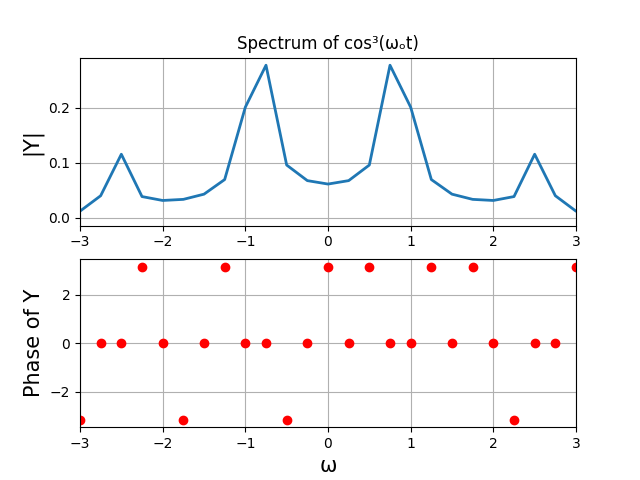
\includegraphics[scale=0.6]{q2.png}
\label{fig:universe}
\end{figure}
\clearpage
The FFT with the hamming Window:
\begin{figure}[h!]
\centering
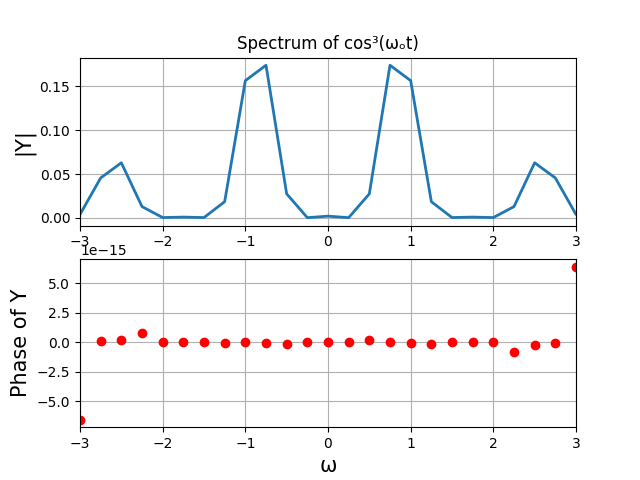
\includegraphics[scale=0.6]{q2(1).png}
\label{fig:universe}
\end{figure}
\clearpage
We notice that a lot of the energy is stored in frequencies that aren't a part of the signal. After windowing, these frequencies are attenuated and hence the peaks are sharper in the windowed function. It is still not an impulse because the convolution with the Fourier transform of the windowed function smears out the peak

\subsection{Question 3}
We need to estimate $\omega$ and $\delta$ for a signal $\cos(\omega t + \delta)$ for 128 samples between $[-\pi,\pi)$. We estimate omega using a weighted average. We have to extract the digital spectrum of the signal and find the two peaks at $\pm\omega_0$, and estimate $\omega$ and $\delta$.
\begin{figure}[h!]
\centering
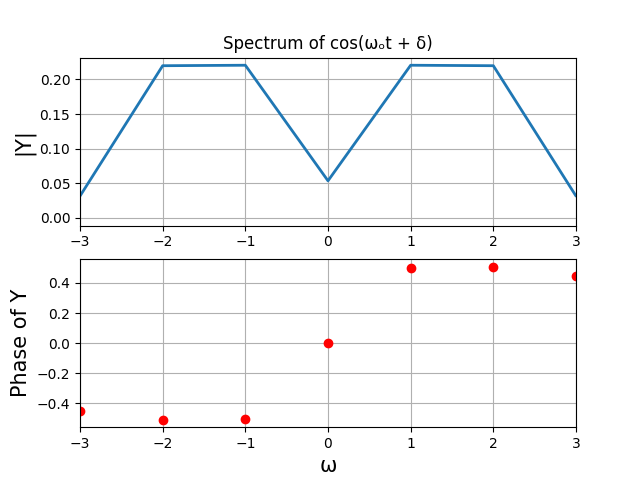
\includegraphics[scale=0.6]{q3.png}
\caption{Fourier transform of $cos(1.5t+0.5)$}
\label{fig:universe}
\end{figure}

We estimate omega by performing a Mean average of $\omega$ over the magnitude of $|Y(j\omega)|$.

For delta we consider a widow on each half of $\omega$ (split into positive and negative values) and extract their mean slope. The intuition behind this is that, a circular shift in the time domain of a sequence results in the linear phase of the spectra.


\subsection{Question 4}
We repeat the exact same process as question 3 but with noise added to the original signal.
\begin{figure}[h!]
\centering
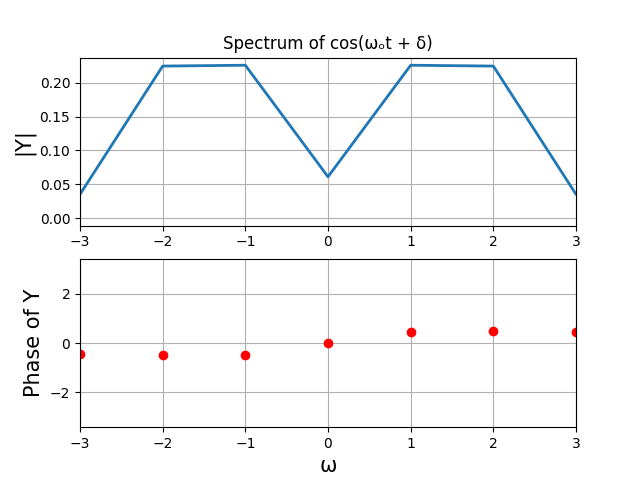
\includegraphics[scale=0.6]{q4.png}
\caption{Fourier transform of noise + $cos(1.5t+0.5)$}
\label{fig:universe}
\end{figure}

For true value of $\omega$ and $\delta$ = 1.5 and 0.5 respectively 
I got :

Omega = 1.5163179648582412\newline
Delta = 0.506776265719626 (in no noisy case)\newline
Omega = 2.0524685950836825\newline
Delta = 0.5009983793316106 (in the noisy case)
\subsection{Question 5}
In this question we analyze a chirp signal which is an FM signal where frequency is directly proportional to time.
A chirp signal we shall consider is given by 
\begin{equation}
    f(t) = cos(16t(1.5 + \frac{t}{2\pi}))
\end{equation}
The FFT of the chirp is given by:
We note that the frequency response is spread between 5-50 rad/s. A large section of this range apears due to Gibbs phenomenon. On windowing, only frequencies between 16 and 32 rad/s remain.
\begin{figure}[h!]
\centering
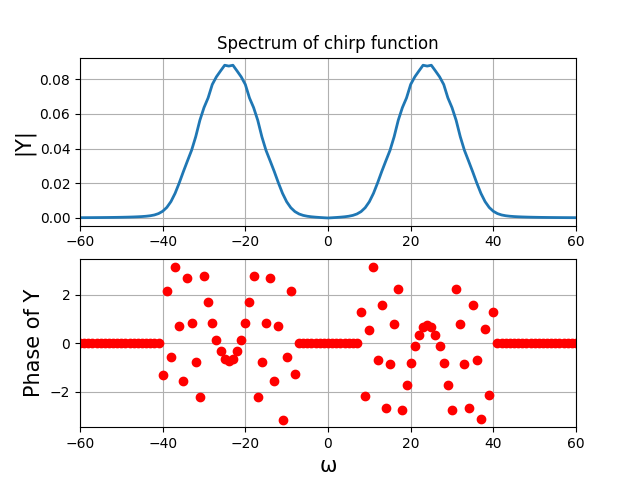
\includegraphics[scale=0.6]{q5(a).png}
\caption{Chirp function fourier transform, windowed}
\label{fig:universe}
\end{figure}
\begin{figure}[h!]
\centering
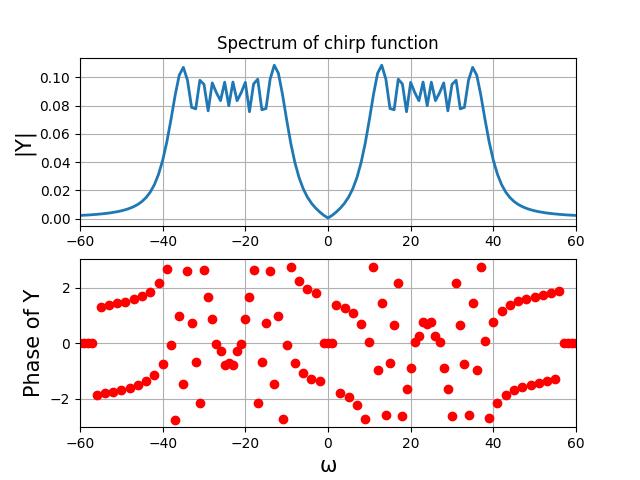
\includegraphics[scale=0.6]{q5(b).png}
\caption{Chirp function fourier transform}
\label{fig:universe}
\end{figure}


\subsection{Question 6}
For the same chirped signal, we break the 1024 vector into pieces that are 64 samples wide.
Extract the DFT of each and store as a column in a 2D array. Then plot the array as a surface plot to show how the frequency of the signal varies with time.
This is new. So far we worked either in time or in frequency. But this is a “time- frequency” plot, where we get localized DFTs and show how the spectrum evolves in time.
We do this for both phase and magnitude. Let us explore their surface plots.

\begin{figure}[h!]
\centering
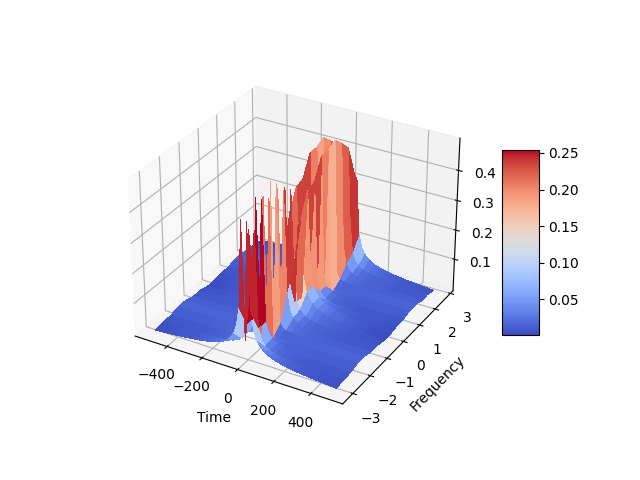
\includegraphics[scale=0.6]{chirp_mag.png}
\caption{Chopped Chirp function, |Fourier transform|}
\label{fig:universe}
\end{figure}

\begin{figure}[h!]
\centering
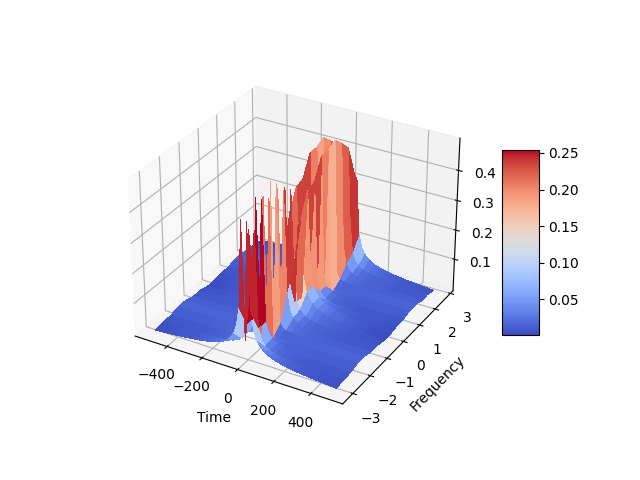
\includegraphics[scale=0.6]{chirp_mag.png}
\caption{Chopped Chirp function, Phase of Fourier transform}
\label{fig:universe}
\end{figure}

\begin{figure}[h!]
\centering
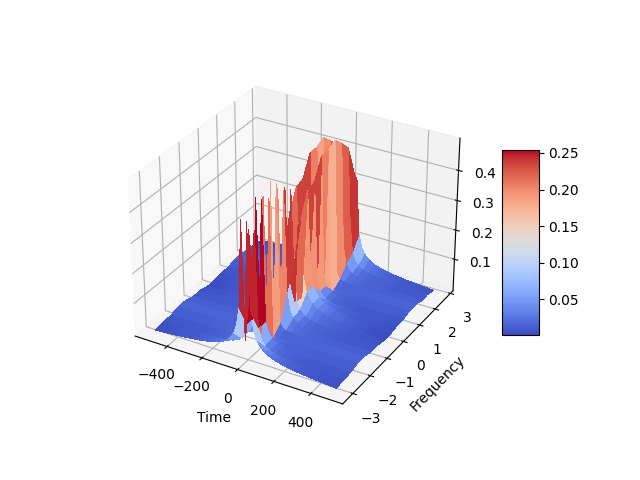
\includegraphics[scale=0.6]{chirp_mag.png}
\caption{Windowed Chopped Chirp function, |Fourier transform|}
\label{fig:universe}
\end{figure}

\begin{figure}[h!]
\centering
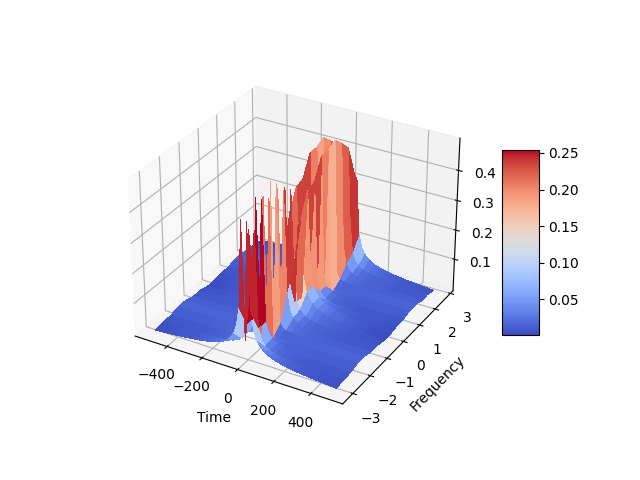
\includegraphics[scale=0.6]{chirp_mag.png}
\caption{Windowed Chopped Chirp function, Phase of Fourier transform}
\label{fig:universe}
\end{figure}


\section{Conclusion}
In this assignment we have covered the requirement of windowing in the case of non-periodic series in DFT's. In particular this is to mitigate the effect of Gibbs phenomena owing to the discontinuous nature of the series $\tilde{x}[n]$ realised by a discrete fourier transform.

The general properties of a fourier spectra for a chirped signal are observable in the time avrying plots , ie..., existence of two peaks (slow growth), vanishing of chirp effects in case of a windowed transform, and a phase plot that periodically varies with reduced phase near maximum values.

The last question addresses the time varying spectra for a chirped signal, where we plot fourier spectra for different time slices of a signal. We noted the case of sparse number of slices and hence took more closely spaced slices.


\end{document}